
\chapter{Diseño del framework}
\label{cap:descripcionTrabajo}
En este capitulo se describe el framework de enemigos creado, mediante el diseño de componentes más sencillos. 
Primero se describirá el contexto y por tanto la utilidad de la herramienta, aquí se detallaran juegos analizados y sus características en común. Después se explicará que elementos la componen y por último se detallarán algunos ejemplos de uso. \\
\section{Descripción general del Framework}
Como se señala en  \citet{Build_a_Bad_Guy_Workshop}, los enemigos bien diseñados son clave para evitar que los niveles queden planos y, en consecuencia, aburridos para el jugador.
Un buen diseño de enemigos va más allá de poner un obstáculo en el camino. Aporta dinamismo, construye la atmósfera del juego y hasta cuenta parte de la historia. Un enemigo puede obligarte a pensar una estrategia específica para vencerlo, o incluso tener una personalidad y comportamientos complejos que hacen que el enfrentamiento sea más significativo e inmersivo. En definitiva, diseñar a los antagonistas es una parte fundamental para crear un juego que enganche y deje huella.\\

El framework se ha diseñado con el objetivo de facilitar la creación de enemigos inteligentes en 2D por medio de comportamientos básicos. Esta orientado a diseñadores, estudiantes o desarrolladores que quieran diseñar comportamientos de enemigos. Con la particularidad de que no es necesario ningún conocimiento de programación.

\subsection{Análisis de enemigos en videojuegos}
El análisis de diversos documentos muestra que la mejor forma de hacer que un enemigo destaque y de un gran potencial al juego es que tenga unos comportamientos únicos. Cada enemigo se define mediante una combinación específica de estos. Determinando así lo que puede y no puede hacer  y permiten diferenciarlo de otros tipos de enemigos. Estos comportamientos han ido evolucionando con el tiempo volviéndose cada vez más sofisticados. Con dicha sofisticación, ha aumentado la complejidad del trabajo en el diseño. Para solucionarlo hemos propuesto una herramienta con comportamientos sencillos y precisos que ayudarán a reducir la carga de trabajo. 

\section{Composición}
En este trabajo, se ha decidido entender como enemigo a cualquier entidad que pueda repercutir de forma negativa en el jugador, esto significa que no se limita el concepto de enemigo a figuras típicas, como monstruos o soldados hostiles, sino que se amplía su definición a toda entidad que suponga un riesgo, dificultad o amenaza para el progreso o el bienestar del jugador dentro del juego, como pueden ser pinchos o lava.
Además separamos cada elemento en función de su comportamiento, implicando que elementos que clásicamente se consideran un único enemigo por aparecer juntos, como la tubería y la gota de ácido o la bala y el pistolero, se tratan aquí como entidades diferentes. Esta decisión se basa en que, desde el punto de vista de la lógica de comportamiento, actúan como elementos autónomos y con reglas distintas.\\

\section{Identificación de comportamientos comunes}
Para poder empezar con el diseño de la herramienta es necesario analizar distintos videojuegos existentes que tengan características comunes al objetivo de la herramienta, en este caso, que sean en dos dimensiones y plataformas.
Para el análisis se estudiaron tres videojuegos. \textit{Hollow Knight} y \textit{Blasphemous} fueron los primeros en analizarse, se hizo un estudio del comportamiento individual de cada enemigo, separando jefes y enemigos comunes y centrándonos en estos últimos. El tercer juego fue \textit{Bzzzt}, que sirvió para verificar que con los comportamientos ya identificados se podría realizar el comportamiento de los enemigos que aparecían con mayor frecuencia en él. 

\subsection{Hollow Knight}
\textit{Hollow Knight} es un \emph{Metroidvania} en 2D desarrollado y auto publicado por el estudio australiano \emph{Team Cherry}\footnote{\url{https://www.teamcherry.com.au/}}. Su versión inicial para ordenador se lanzó en 2017. El jugador controla al \textit{Caballero}, que explora un reino subterráneo de insectos abandonado. Derrotando enemigos por medio de distintas habilidades que se van desbloqueando, se descubre el mundo y los secretos que este oculta.

\subsection{Blasphemous}
Desarrollado por el estudio sevillano \emph{The Game Kitchen}\footnote{\url{https://thegamekitchen.com/}} y publicado por Team17, \textit{Blasphemous}\footnote{\url{https://thegamekitchen.com/blasphemous/}} llegó a Windows, Nintendo Switch, PlayStation 4 y Xbox One el 10 de septiembre de 2019. El jugador encarna al \textit{Penitente} el único superviviente en la tierra de Cvstodi. Atrapado en un ciclo de penitencia de muerte y resurrección, el Penitente tendrá que liberar al mundo del destino que le espera.

\subsection{Bzzzt}

\textit{Bzzzt}\footnote{\url{https://store.steampowered.com/app/1293170/BZZZT/}} es un plataformas de acción de estética retro desarrollado casi íntegramente por el checo Karel Matějka  y publicado por Cinemax. Se estrenó para PC en noviembre de 2023 y para Nintendo Switch en septiembre de 2024. el jugador, en el papel de un robot, debe frustrar los planes del villano Badbert y rescatar a sus creadores, los doctores Emily y Norbert, atravesando 52 niveles llenos de trampas y enemigos de estilo arcade.

\subsection{Comportamientos relevantes detectados}
El análisis de los juegos permitió la identificación de los siguientes patrones:  
\begin{itemize}
  \item \emph{Patrulla:} Este comportamiento se caracteriza por caminar a un ritmo constante en el eje horizontal, cambiando de dirección al chocar. Se identificó en los tres juegos y en distintos enemigos dentro de cada uno de ellos (p.\,ej., Reptacillo del Hollow Knight (Figura \ref{fig:Reptacillo})).  
  \item \emph{Torreta:} Enemigos que lanzan proyectiles de forma periódica  (p.\,ej., Vengamosca antes de moverse).  
  \item \emph{Embate lineal:} Consiste en una vez detectado al jugador modificar significativamente la velocidad, aumentándola para atacarle. (p.\,ej., Cáscara errante).  
  \item \emph{Aparición del suelo:} Son enemigos que parece que están saliendo del suelo, no atacan, solo salen y se esconden (p.\,ej., Goam o pinchos ).  
  \item \emph{Persecución:} Son enemigos que persiguen al jugador hasta chocarse con él. La persecución se puede dar de distintas formas, unicamente en un eje o si el enemigo vuela, en forma de revolotéo donde no se acerca directamente si no que va deambulando.
  \item \emph{Rotación:} Estos describen un movimiento circular alrededor de un punto (p.\,ej. Bolas circulares de Bzzzt).
  \item \emph{Seguimiento de camino:} Enemigos que siguen un camino predeterminado y no lo abandonan independientemente del jugador (p.\,ej. Balas de Bzzzt).
\end{itemize}

\begin{figure}[t]
	\centering
	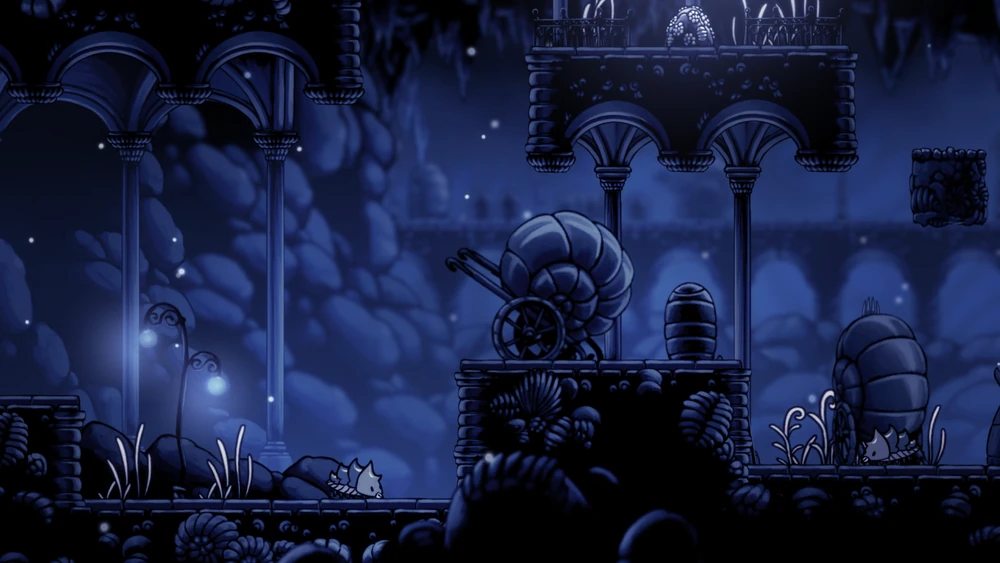
\includegraphics[height=5cm]{Imagenes/Reptacillo_Image.png}
	\caption{Imagen de escenario de \textit{Hollow Knight} donde aparecen dos Reptacillos}
	\label{fig:Reptacillo}
\end{figure}

\section{Actuadores}
\label{subsec:acciones}
Hace referencia a un conjunto de movimientos y habilidades que definen lo que un enemigo puede hacer en el videojuego. Esto incluye distintos tipos de desplazamientos y la capacidad de crear otros enemigos de forma independiente (spawners). Estas habilidades no siempre son compatibles entre sí, teniendo una tabla en la que se indicaran las relaciones entre ellas. Además no es necesario utilizar siempre todas las acciones de forma que a veces un enemigo podrá realizar un tipo de movimiento o usar un spawner de manera exclusiva, mientras que en otras podrá combinar varias habilidades según su diseño y complejidad. Esto permite adaptar las capacidades de los enemigos para diferentes situaciones en el juego.

\subsection{Movimiento}
Podemos definir el término movimiento como el desplazamiento o cambio de posición de un enemigo dentro del juego. Sin embargo, el concepto de movimiento también puede aplicarse en el caso de enemigos que permanecen en una posición fija, haciendo referencia a la ausencia de éste. Los movimientos son fundamentales para definir el comportamiento de los personajes, ya que permiten la interacción con el jugador y el entorno.\\

A continuación se muestran todos los movimientos diseñados, junto con una breve descripción.
\begin{itemize}
  \item \textbf{Horizontal}: Desplaza al enemigo horizontalmente, hacia la izquierda o derecha.
    \item \textbf{Vertical}: Desplaza al enemigo verticalmente, hacia arriba o abajo.
    \item \textbf{Directional}: Mueve al enemigo en una dirección definida por un ángulo, siendo el valor cero un movimiento hacia la derecha e incremental en el sentido antihorario.
    \item \textbf{Circular}: Hace que el enemigo siga un movimiento circular alrededor de un punto, describiendo una circunferencia cerrada si el ángulo es igual a 360 y, en caso de ser menor, actuando como péndulo.
    \item \textbf{Move To A Point}\label{sec:MoveToAPoint}: Dirige al enemigo hacia puntos concretos no actualizables. Se puede configurar por medio de una lista, donde se indican los puntos concretos a recorrer o por medio de un área, donde se eligirá aleatoriamente un punto y al llegar a él, se escogerá otro.
    \item \textbf{Move To An Object}: Desplaza al enemigo hacia una entidad que puede estar en movimiento.
    \item \textbf{Spline Follower}: Permite al enemigo seguir una trayectoria definida por una curva suave que se genera a partir de un conjunto de puntos de control (spline).
\end{itemize}

Todos los tipos de movimiento pueden configurarse para ejecutarse de forma acelerada. Para ello, se emplea una función de aceleración/suavizado ( \textit{Easing Function}), una función que define cómo varían en un tiempo definido tanto la velocidad como la posición del enemigo. \\
Dependiendo del tipo de movimiento, esta función puede aplicarse de dos formas:\\

\begin{itemize}
\item En movimientos como \textbf{Horizontal}, \textbf{Vertical}, \textbf{Directional} o \textbf{Circular}, la \textit{Easing Function} afecta principalmente a la velocidad, modificándola teniendo en cuenta una velocidad objetivo y un tiempo para llegar a ella.
\item En movimientos como \textbf{Move To A Point} y \textbf{Move To An Object} (Figura \ref{fig:EasingFunction}), la \textit{Easing Function} influye directamente en la interpolación de la posición, alterando cómo el enemigo se desplaza entre el origen y el destino en un tiempo determinado.
\end{itemize}

Este enfoque permite controlar el dinamismo del movimiento, proporcionando una mayor expresividad y naturalidad en el comportamiento de los enemigos. Por ello, se incluye un catálogo\footnote{\url{https://gist.github.com/cjddmut/d789b9eb78216998e95c}} de distintas \textit{Easing Functions} que permite variar la forma en que se definen y perciben los movimientos.\\

La manera en la que influyen las \textit{EasingFunction} en cada tipo de movimiento será explicada con más profundidad en el apartado de Implementación (Capítulo \ref{cap:implementacion}).

\begin{figure}[t]
	\centering
	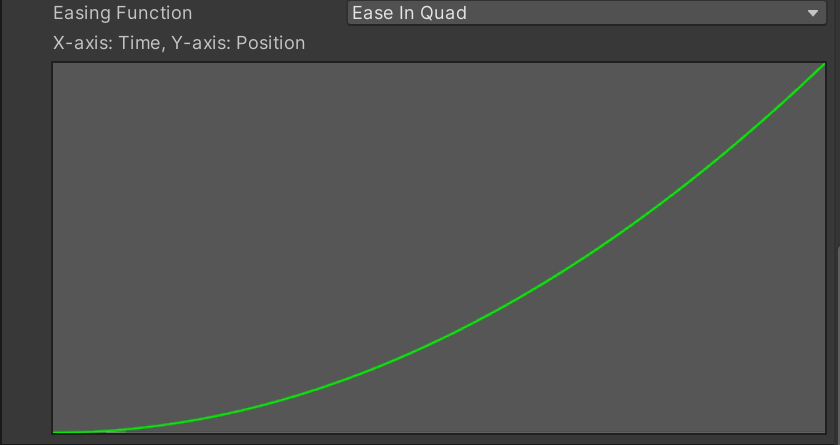
\includegraphics[height=5cm]{Imagenes/EasingFunction.png}
	\caption{Easing Function que describe la variación de la posición de un objeto con el movimiento \textbf{Move To An Object}}
	\label{fig:EasingFunction}
\end{figure}

\subsection{Spawner}
Capacidad que poseen los enemigos para generar otros enemigos independientes, es decir, poder crear nuevas unidades que actúan de forma autónoma dentro del juego. Un ejemplo serían las torretas, que crean balas.\\

Implementar un spawner requiere establecer ciertas reglas de generación de enemigos, tales como la frecuencia de aparición o el número máximo de enemigos generados.
\subsection{Compatibilidad}
La versatilidad de la herramienta se potencia al permitir la combinación de diversos actuadores simultáneamente. En este sentido, un enemigo podría perfectamente desplazarse horizontalmente mientras activa un spawner para generar secuaces. Esta sinergia entre actuadores (movimientos y spawners) enriquece la complejidad del comportamiento y abre un abanico de posibilidades creativas para los diseñadores.\\

No obstante, es crucial reconocer que no todas las combinaciones de acciones resultan coherentes o deseables desde la perspectiva del diseño del juego. Por ejemplo, intentar realizar un movimiento vertical mientras se está definido un movimiento circular podría generar comportamientos visuales o de jugabilidad no intencionados. \\

Para clarificar estas interdependencias y asegurar la coherencia en la configuración de los enemigos, se ha elaborado la tabla \textbf{tabla~\ref{tab:compatibilidad}} de compatibilidad. Esta tabla actuará como una guía visual e intuitiva, indicando qué combinaciones de movimientos y la activación de spawners son factibles y recomendadas, permitiendo a los diseñadores construir enemigos con comportamientos complejos pero lógicos y bien definidos.

\begin{table}[!h]
    \centering
    \caption{Matriz de compatibilidad de movimientos}
    \label{tab:compatibilidad}
    \resizebox{\textwidth}{!}{%
    \begin{tabular}{|l|c|c|c|c|c|c|c|c|}
    \hline
    \textbf{} & \textbf{Horizontal} & \textbf{Vertical} & \textbf{Directional} & \textbf{Circular} & \textbf{Move To A Point} & \textbf{Move To An Object} & \textbf{Spline Follower} & \textbf{Spawner} \\
    \hline
    \textbf{Horizontal} & \cellcolor{gray!40} & \cellcolor{gray!40} & \cellcolor{gray!40} & \cellcolor{gray!40} & \cellcolor{gray!40} & \cellcolor{gray!40} & \cellcolor{gray!40} & \cellcolor{gray!40} \\
    \hline
    \textbf{Vertical} & \cellcolor{green!70} & \cellcolor{gray!40} & \cellcolor{gray!40} & \cellcolor{gray!40} & \cellcolor{gray!40} & \cellcolor{gray!40} & \cellcolor{gray!40} & \cellcolor{gray!40} \\
    \hline
    \textbf{Directional} & \cellcolor{red!70} & \cellcolor{red!70} & \cellcolor{gray!40} & \cellcolor{gray!40} & \cellcolor{gray!40} & \cellcolor{gray!40} & \cellcolor{gray!40} & \cellcolor{gray!40} \\
    \hline
    \textbf{Circular} & \cellcolor{red!70} & \cellcolor{red!70} & \cellcolor{red!70} & \cellcolor{gray!40} & \cellcolor{gray!40} & \cellcolor{gray!40} & \cellcolor{gray!40} & \cellcolor{gray!40} \\
    \hline
    \textbf{Move To A Point} & \cellcolor{red!70} & \cellcolor{red!70} & \cellcolor{red!70} & \cellcolor{red!70} & \cellcolor{gray!40} & \cellcolor{gray!40} & \cellcolor{gray!40} & \cellcolor{gray!40} \\
    \hline
    \textbf{Move To An Object} & \cellcolor{red!70} & \cellcolor{red!70} & \cellcolor{red!70} & \cellcolor{red!70} & \cellcolor{red!70} & \cellcolor{gray!40} & \cellcolor{gray!40} & \cellcolor{gray!40} \\
    \hline
    \textbf{Spline Follower} & \cellcolor{red!70} & \cellcolor{red!70} & \cellcolor{red!70} & \cellcolor{red!70} & \cellcolor{red!70} & \cellcolor{red!70} & \cellcolor{gray!40} & \cellcolor{gray!40} \\
    \hline
    \textbf{Spawner} & \cellcolor{green!70} & \cellcolor{green!70} & \cellcolor{green!70} & \cellcolor{green!70} & \cellcolor{green!70} & \cellcolor{green!70} & \cellcolor{green!70} & \cellcolor{gray!40} \\
    \hline
    \end{tabular}
    }
\end{table}
\section{Sensores}
\label{subsec:sensores}
El término sensor se define como los mecanismos mediante los cuales los personajes interactúan con su entorno y entre sí.
Podemos definir el término sensor como el elemento que sirve para que el enemigo conozca el entorno y reciba información de los cambios que se producen en el mismo. Son los responsables de activar las transiciones entre estados, es decir, se encargan de cambiar de un comportamiento predefinido a otro.
A continuación se enumerarán los diferentes sensores disponibles en la herramienta.
\begin{itemize}
    \item \textbf{Area}: Detecta si un objeto entra o sale en una zona de detección.
    \item \textbf{Collision}: Detecta colisiones físicas con otros objetos.
    \item \textbf{Distance}: Detecta si un objeto está dentro o fuera de una distancia específica.
    \item \textbf{Time}: Detecta cuando ha transcurrido un tiempo determinado.
\end{itemize}
\section{Daño}
Se define daño como la consecuencia negativa que recibe una entidad con respecto a su vida. Esto se produce como la consecuencia de una colisión entre dos entidades del juego, una que hace daño y otra que lo recibe.\\
Existen diferentes tipos de daño y parámetros específicos que determinan cómo las entidades reciben, emiten y procesan daño.
La primera consideración que hay que tener en cuenta es que el daño no es bidireccional, lo que implica que un volumen que recibe daño no tiene por qué emitir daño. Para reflejar esta diferenciación se han creado los siguientes dos componentes:
\begin{itemize}
    \item \textbf{Damage Sensor}: Detecta si el objeto ha recibido daño.
    \item \textbf{Damage Emitter}: Efectúa daño.
\end{itemize}

Además, se puede distinguir entre tres tipos de daños:
\begin{itemize}
    \item \textbf{Instantáneo:} Aplica una única vez el daño al tener contacto.
    \item \textbf{De Permanencia:} Inflige daño continuo mientras haya contacto, definiendo la cantidad y la frecuencia de aplicación de daño.
    \item \textbf{Residual:} Aplica daño inicial y luego daño periódico tras el contacto, definiendo cantidades, frecuencia de aplicación y número de aplicaciones.
\end{itemize}

\section{Estado}
\label{subsec:estado}

Un estado se define como un conjunto específico de acciones. Esta conjunción de elementos define de manera integral la conducta observable del enemigo en un momento dado. Las acciones que un estado puede englobar comprenden uno o varios tipos de movimiento que resulten compatibles entre sí, permitiendo una ejecución coordinada de desplazamientos. Adicionalmente, un estado puede tener la capacidad de generar nuevas entidades enemigas a través de un mecanismo de instanciación (spawner), enriqueciendo la dinámica y la complejidad del entorno de juego. 

\section{Máquina de estados finita}

La Máquina de Estados Finita (FSM, Finite State Machine) es el núcleo de la lógica que define el comportamiento de los enemigos en nuestro diseño. Cada enemigo tiene su propia FSM, configurada específicamente para representar sus patrones de acciones, reacciones y relaciones en el juego. La FSM organiza el comportamiento de los enemigos mediante estados y transiciones:
Los estados, como ya se ha explicado, agrupan las acciones que el enemigo puede realizar en un momento dado.
Las transiciones permiten cambiar de un estado a otro y son activadas por sensores.\\

\begin{figure}[t]
	\centering
	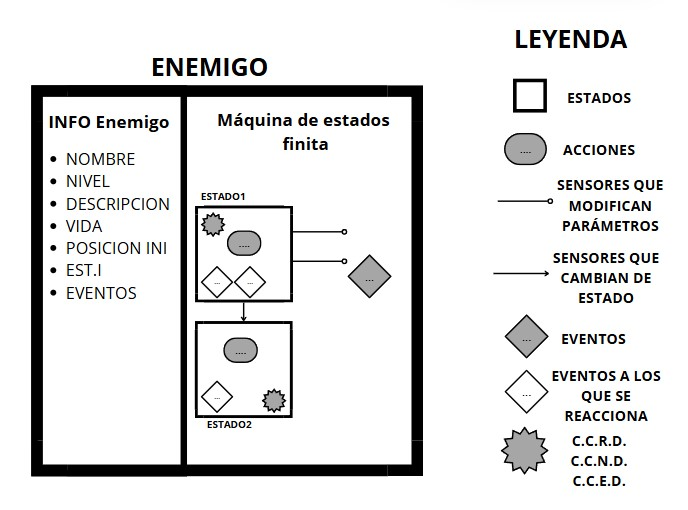
\includegraphics[height=5cm]{Imagenes/EnemigoGeneral.png}
	\caption{Enemigo General }
	\label{fig:EnemigoGeneral}
\end{figure}

\section{Ejemplos de uso}
Con esta separación de actuadores, sensores y daño la creación de enemigos se vuelve mucho más sencilla. A continuación se presentan unos ejemplos construidos mediante la combinación de los componentes de la herramienta sin la necesidad de escribir código, estos ejemplos están incluidos en la propia herramienta.\\


Se mencionarán algunos componentes que aún no han sido introducidos, estos serán explicados en el Capítulo \ref{cap:implementacion}.\\


Todos los enemigos mencionados incluyen los siguientes componentes:

\begin{itemize}
\item Un \texttt{Animator Controller} propio, configurado de manera que las animaciones se correspondan con la lógica de comportamiento de cada enemigo.
\item Un componente de tipo \texttt{FSM} (Finite State Machine).
\item Al menos un componente de tipo \texttt{State}. Siempre que se mencione que un enemigo incorpora un \texttt{Actuator}, \texttt{Sensor} o \texttt{DamageEmitter}, estos estarán referenciados dentro de una clase \texttt{State} específica. En caso de no especificarse ninguna, se asumirá que el enemigo dispone de un único estado.
\end{itemize}

\subsection{Bouncing Bunny}

En la Figura \ref{fig:BouncingBunny} se puede ver un enemigo sencillo utilizado habitualmente al comienzo de los juegos de plataformas en dos dimensiones. El enemigo se desplaza de izquierda a derecha describiendo un movimiento horizontal, hasta colisionar con una pared, momento en el cual cambia de dirección.\\

Para construir este comportamiento, configuramos un único estado el cual tiene un \texttt{Horizontal Actuator} configurado para que rebote en caso de colisionar con las paredes y con una velocidad constante y un \texttt{Damage Emitter} configurado para realizar daño instantáneo, concretamente una única unidad.\\

También necesitaremos añadir un componente \texttt{Life} configurado para que el enemigo tenga un punto de vida.

\begin{figure}[t]
	\centering
	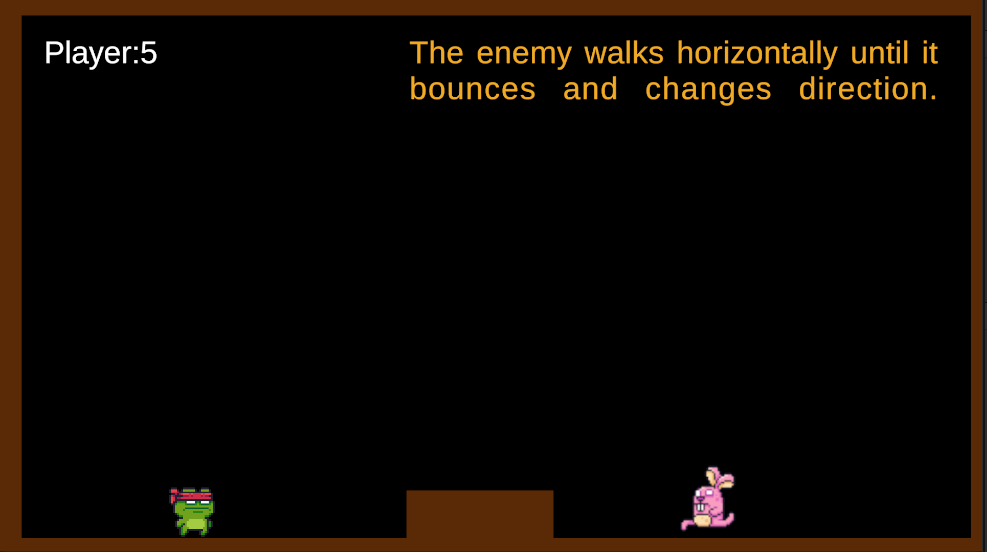
\includegraphics[height=5cm]{Imagenes/BouncingBunny.png}
	\caption{Escena de ejemplo donde observamos al enemigo en cuestión momentos antes de alcanzar la pared.}
	\label{fig:BouncingBunny}
\end{figure}

\subsection{Spinning Rocks}

Con respecto al enemigo mostrado en la Figura~\ref{fig:SpinningRocks}, este realiza un movimiento circular alrededor de un punto central. Aunque en apariencia pueda parecer una única entidad, en realidad cada bola actúa como un enemigo independiente que ejecuta su propio movimiento circular.\\

Este tipo de enemigo no puede ser detenido ni eliminado en ningún momento, por lo que no tendrá componente relacionado con la vida, lo que incrementa significativamente su nivel de peligrosidad. Su presencia constante y la imposibilidad de neutralizarlo lo convierten en una amenaza persistente dentro del escenario de juego.\\

Para construirlo necesitaremos crear tres objetos con los sprites mostrados en la figura con un \texttt{Circular Actuator} con los parámetros necesarios para que produzca un giro completo de \textit{360º}. También necesitará un \texttt{Damage Emitter} configurado para realizar daño instantáneo, concretamente una única unidad.\\

Cada objeto necesitará asignar un punto sobre el que rotar, por lo que se necesitará crear otro objeto que sirva como centro de la rotación.\\

\begin{figure}[t]
	\centering
	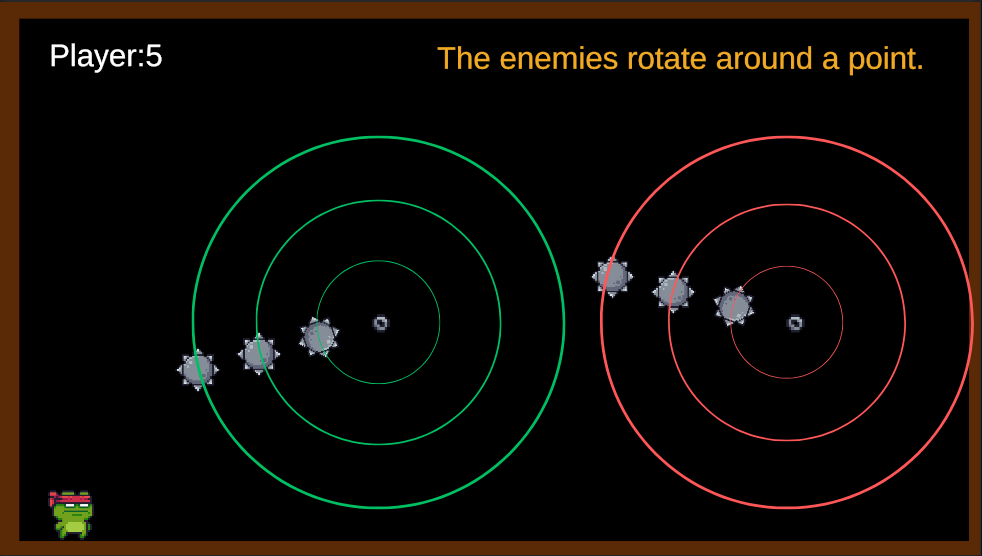
\includegraphics[height=5cm]{Imagenes/SpinningRocks.png}
	\caption{Escena de ejemplo donde se aprecian dos enemigos realizando un movimiento circular cada uno en un sentido diferente}
	\label{fig:SpinningRocks}
\end{figure}

\subsection{Trunk Torret}

Con respecto al enemigo mostrado en la Figura~\ref{fig:TrunkTurret}, este permanece completamente estático durante toda su existencia en el escenario. A pesar de su falta de movilidad, representa una amenaza constante al disparar proyectiles de manera periódica cada dos segundos, lo que obliga al jugador a mantenerse en movimiento para esquivarlos.\\

Este enemigo es completamente invulnerable  a cualquier tipo de ataque y tampoco hace daño directamente, por lo que no cuenta con componentes asociados a vida o daño, tanto recibido como realizado. Esta característica aumenta su peligrosidad, ya que su presencia no puede ser eliminada y el jugador debe enfrentarse a él únicamente mediante la evasión.\\

Para implementarlo, se le asignará un componente de tipo \texttt{Spawner Actuator}, configurado para emitir un proyectil cada dos segundos que aparece desde un punto de su boca.
\subsubsection{Bullet}

El proyectil generado por la \textit{Trunk Turret} se desplaza horizontalmente hacia la izquierda con un movimiento lineal. Al entrar en contacto con el jugador, produce daño instantáneo. En caso de colisionar con el entorno o con el propio jugador, el proyectil se destruirá automáticamente.\\

Para construir este comportamiento, se utilizará un objeto , al que se le asignará un \texttt{Horizontal Actuator} configurado para el movimiento en dirección izquierda y que reaccione al contacto destruyéndose, así como un \texttt{Damage Emitter} capaz de infligir una unidad de daño al contacto. 


\begin{figure}[t]
	\centering
	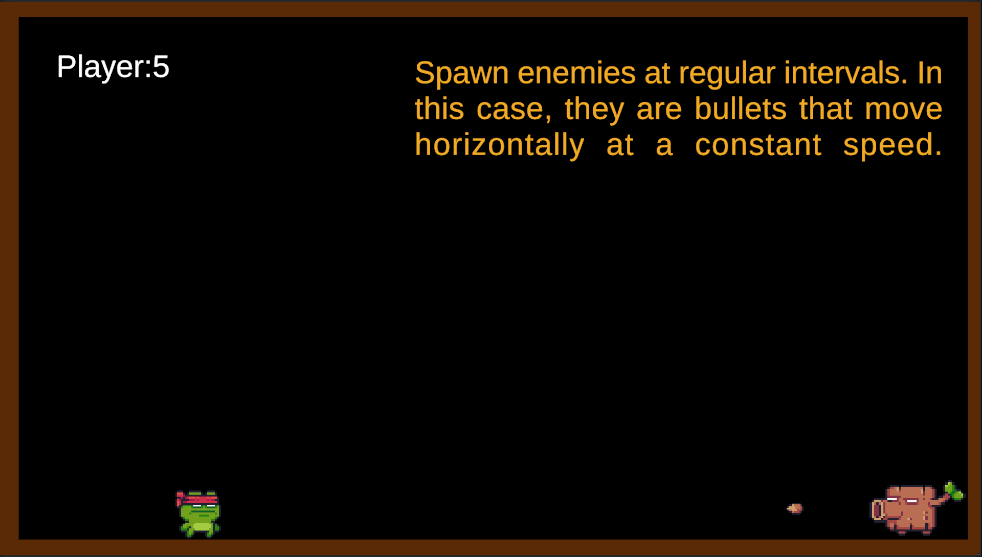
\includegraphics[height=5cm]{Imagenes/TrunkTorret.png}
	\caption{Escena de ejemplo donde se aprecia una \textit{TrunkTorret} disparando.}
	\label{fig:TrunkTurret}
\end{figure}
\subsection{Spline Chicken}

Con respecto al enemigo mostrado en la Figura~\ref{fig:SplineChicken}, esta gallina realiza un movimiento continuo siguiendo una trayectoria curva predefinida (spline) que rodea una plataforma. Este desplazamiento suave y cerrado permite que patrulle una zona concreta, dificultando el paso del jugador y añadiendo presión durante momentos clave del recorrido.\\

Aunque su apariencia pueda resultar cómica o inofensiva, este enemigo representa una amenaza real, ya que inflige daño al contacto. Además, no puede ser eliminado ni detenido, lo que lo convierte en un obstáculo constante que obliga al jugador a calcular cuidadosamente el momento en el que atravesar su recorrido.\\

Para su implementación, se instanciará un objeto con el sprite correspondiente, al que se le añadirá un componente de tipo \texttt{Spline Follower}, configurado para recorrer una trayectoria cerrada en bucle. Además, se incluirá un \texttt{Damage Emitter} que provocará la eliminación instantánea del jugador.\\

Tendrá un componente \texttt{Life}.

\begin{figure}[t]
	\centering
	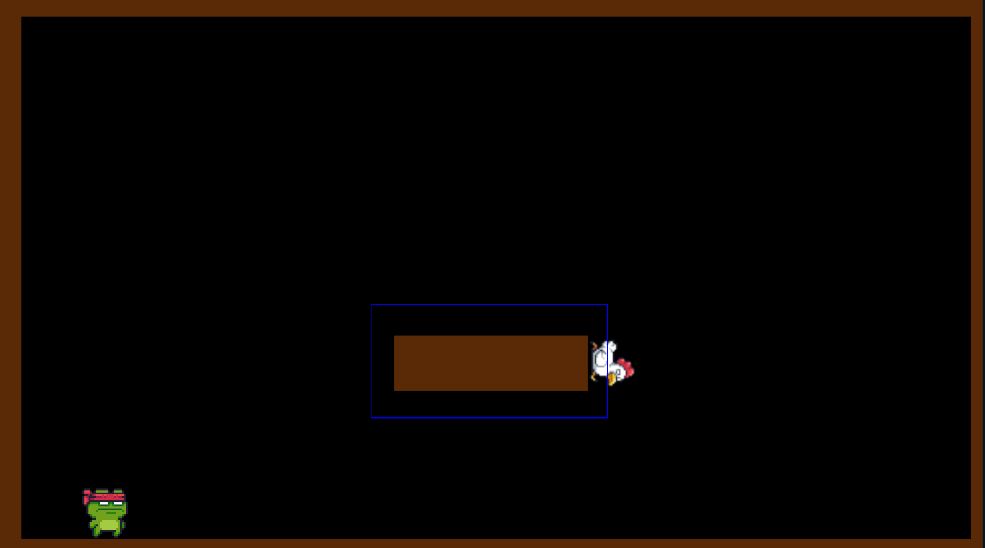
\includegraphics[height=5cm]{Imagenes/Gallina_Spline.png}
	\caption{Escena de ejemplo donde se aprecia una \textit{Spline Chicken} siguiendo su trayectoria.}
	\label{fig:SplineChicken}
\end{figure}

\subsection{Skywatch Eagle}

Con respecto al enemigo mostrado en la Figura~\ref{fig:SkywatchEagle}, este águila deambula libremente por una zona delimitada del escenario, describiendo un patrón de patrullaje aéreo. Su comportamiento cambia de forma agresiva en cuanto detecta la presencia del jugador dentro de su campo de visión, momento en el cual se lanza en picado a gran velocidad con la intención de impactarlo.\\

Este enemigo combina movilidad impredecible y comportamiento reactivo, lo que lo convierte en una amenaza considerable. Su capacidad para alterar su trayectoria bruscamente en función de la posición del jugador obliga a mantenerse en constante movimiento y a anticipar su patrón de ataque.\\

Para construir este comportamiento, se utilizarán un componentes de tipo \texttt{State} extra:

\begin{itemize}
\item Uno de ellos será el comportamiento de patrulla, estado en el que el enemigo se desplaza aleatoriamente por una zona aérea mediante un \texttt{Move To A Point Actuator} configurado para moverse a través de puntos generados aleatoriamente en la zona gris de la  Figura~\ref{fig:SkywatchEagle}. En este estado también se encuentra la transición al estado de ataque, a través de un \texttt{Distance Sensor} que mide la distancia entre ambos. \\
\item En este estado, el águila se mueve rápidamente hacia la posición del jugador usando un \texttt{Move To Object Actuator}. Cuando el daño es realizado, vuelve a su estado inicial a través de un \texttt{Collision Sensor} configurado para activarse al contacto con el jugador.
\end{itemize}

Adicionalmente, contará con un \texttt{Damage Emitter} que inflige una unidad de daño si colisiona con el jugador durante el picado y exclusivamente durante el picado.
\begin{figure}[t]
	\centering
	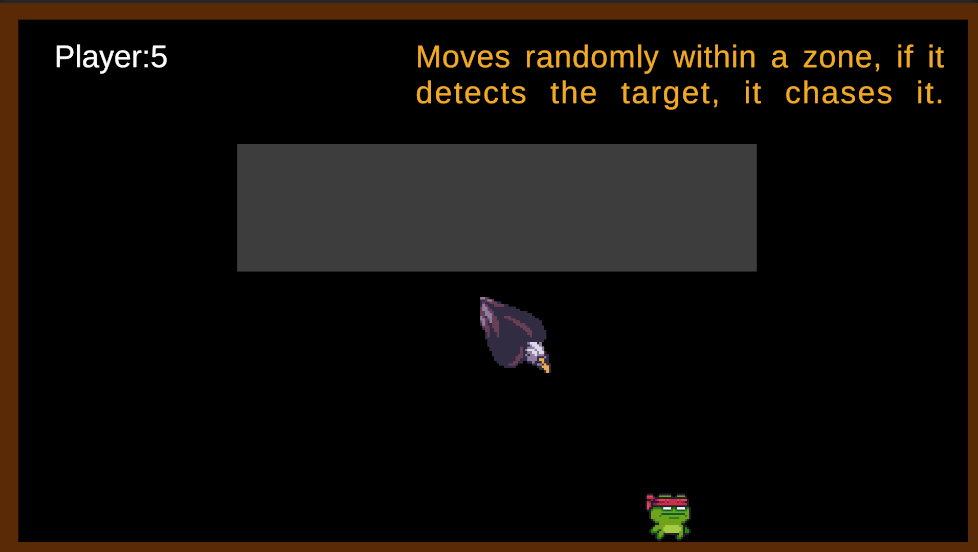
\includegraphics[height=5cm]{Imagenes/AguilaCayendo.png}
	\caption{Escena de ejemplo donde se aprecia a la \textit{Skywatch Eagle} atacando al jugador.}
	\label{fig:SkywatchEagle}
\end{figure}


